
 
\subsection{Visualizing the convolution kernels} \label{sec:visualize_operator}
As seen in the previous sections, all the kernels separate into a part which depends only on the angular distance between pixels and another part that depends on the azimuthal orientation around the central pixel. The radial part of the kernels determines the non-locality of the operator. 
We numerically compute the radial kernels: $f, _{+2}f ~\&~ _{-2}f $ by evaluating the respective multipole sums given in \eq{eq:rad_ker_queb} and \eq{eq:f2_rad_ker} in the band limit $\ell \in [=2,192]$. The resultant functions are depicted in \fig{fig:beta_kernel}. 
%
\begin{figure}[!hbt]
\centering
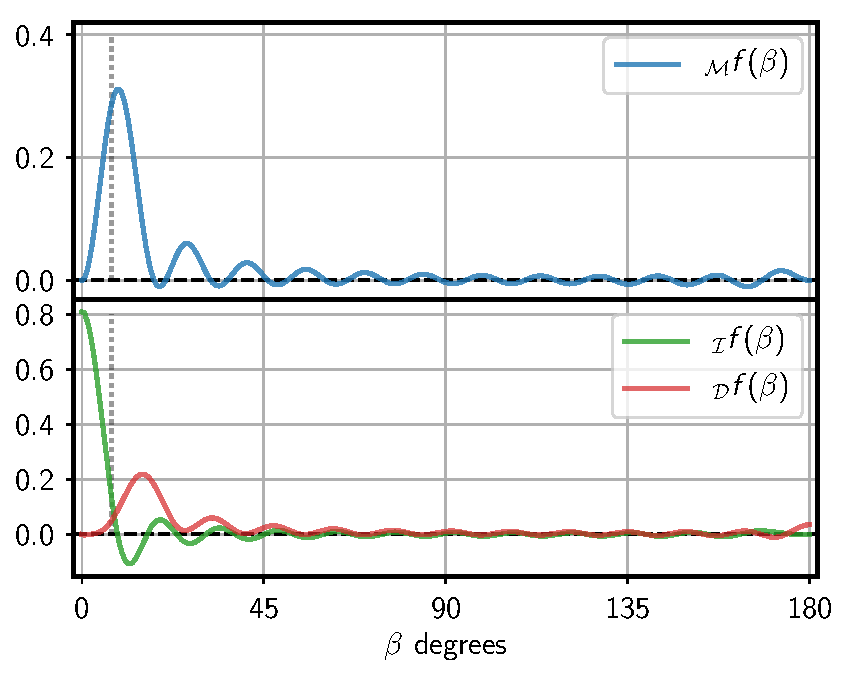
\includegraphics[width=0.8\columnwidth]{kernel/beta_kernel.pdf}
\caption{The figure depicts the radial part of the convolution kernels. These radial function have been evaluated with the band limit fixed at $\ell \in [2,192]$. The vertical dashed line marks the approximate size of a NSIDE=64 Healpix pixel.}
\label{fig:beta_kernel}
\end{figure}
%
Note that the function $f(\beta)$, which forms the radial part of the real space convolution kernel that translates the Stokes parameters Q \& U to scalars E \& B, has a vanishing contribution from the location of the central pixel ($\beta \rightarrow 0$). Recall that the fields E \& B are scalar and hence expected to be immune to coordinate definitions. The locally defined Stokes parameters however necessarily depend on the coordinate definition. Therefore, this nature of the radial kernel is to be expected in order for it to satisfy the requirement of the derived quantities being coordinate independent. 

The functions $_{+2}f(\beta)~\&~_{-2}f(\beta)$, both contribute to the convolution kernels which decompose the Stokes parameters into those corresponding to the respective scalar modes E \& B. $_{-2}f(\beta)$ form the radial part of the band limited delta function $I$ and hence it contributes the most at the location of the central pixel. $_{+2}f(\beta)$ again has a vanishing contribution near the central pixel and it dominantly contributes in the neighbouring regions which are approximately at least 1 pixel distance away from the central pixel.

The azimuthal dependencies of the convolution kernels, are specified as functions of the Euler angles $\alpha ~\&~ \gamma$. We evaluate the real and imaginary parts of the functions $\mathcal{M}, \mathcal{D}~\&~\mathcal{I}$ by calculating the Euler angles for all the pixels surrounding the central pixel and using them in \eq{eq:op_qu2eb}, \eq{eq:fn_i} and \eq{eq:fn_d} respectively.
 %
\begin{figure}[t] \label{fig:mixing_kernel}
\centering
%\captionsetup[subfigure]{labelformat=empty}
\subfigure{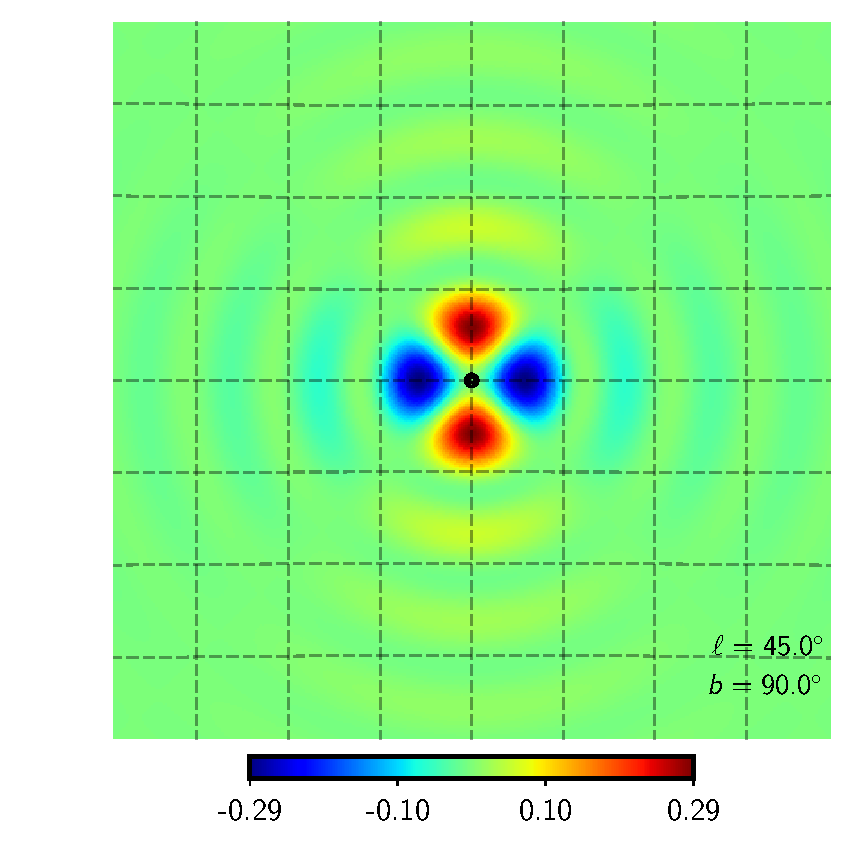
\includegraphics[width=0.16\columnwidth]{kernel/qu2eb_ker_r_lat90_lon45.pdf}}\hspace{-2mm}
\subfigure{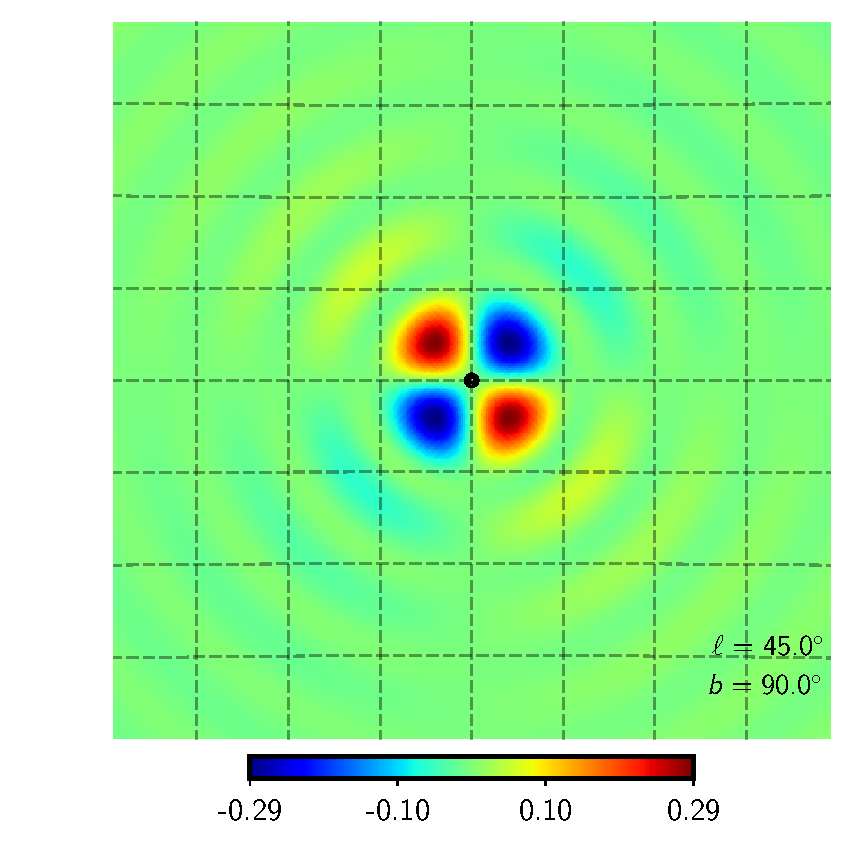
\includegraphics[width=0.16\columnwidth]{kernel/qu2eb_ker_i_lat90_lon45.pdf}}\hspace{-2mm}
\subfigure{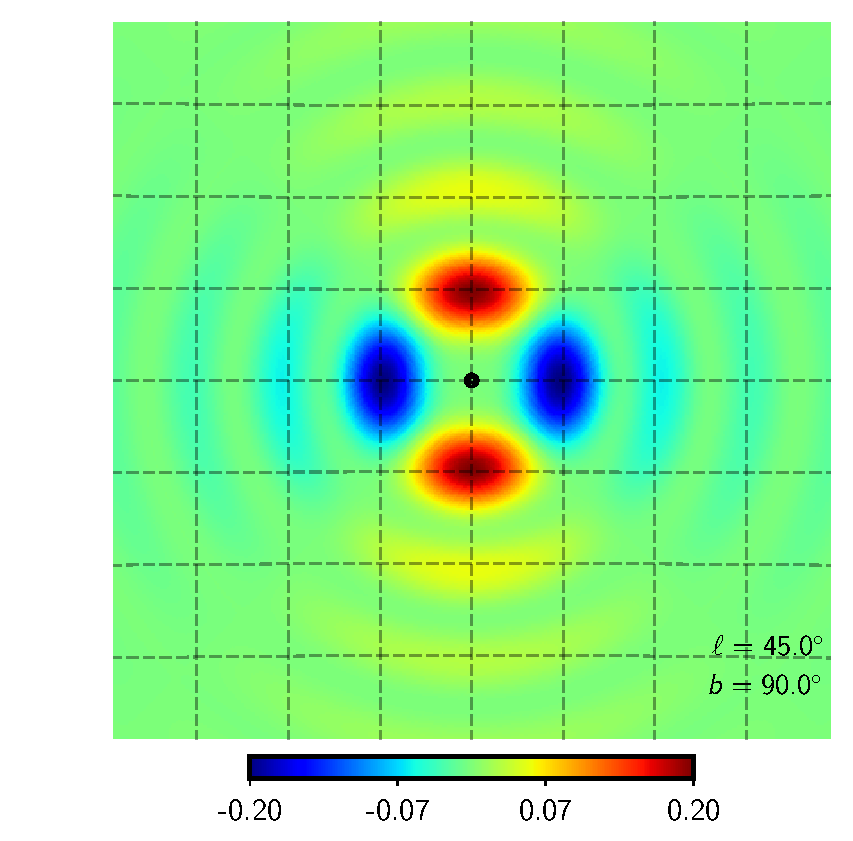
\includegraphics[width=0.16\columnwidth]{kernel/qu2ebqu_ker_r_lat90_lon45.pdf}}\hspace{-2mm}
\subfigure{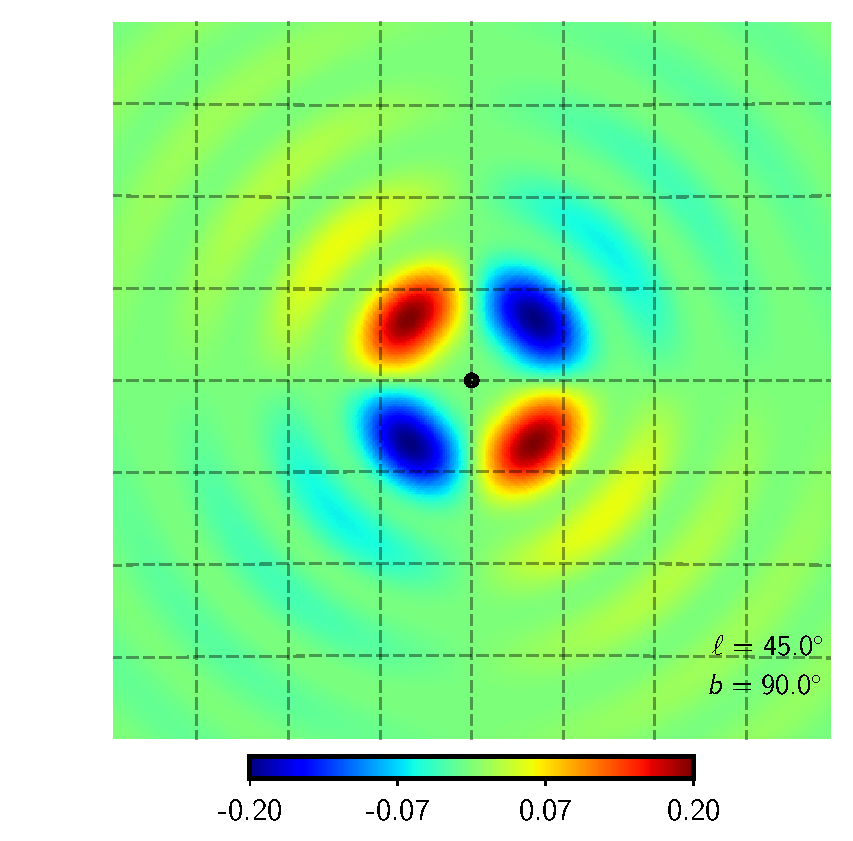
\includegraphics[width=0.16\columnwidth]{kernel/qu2ebqu_ker_i_lat90_lon45.pdf}}\hspace{-2mm}
\subfigure{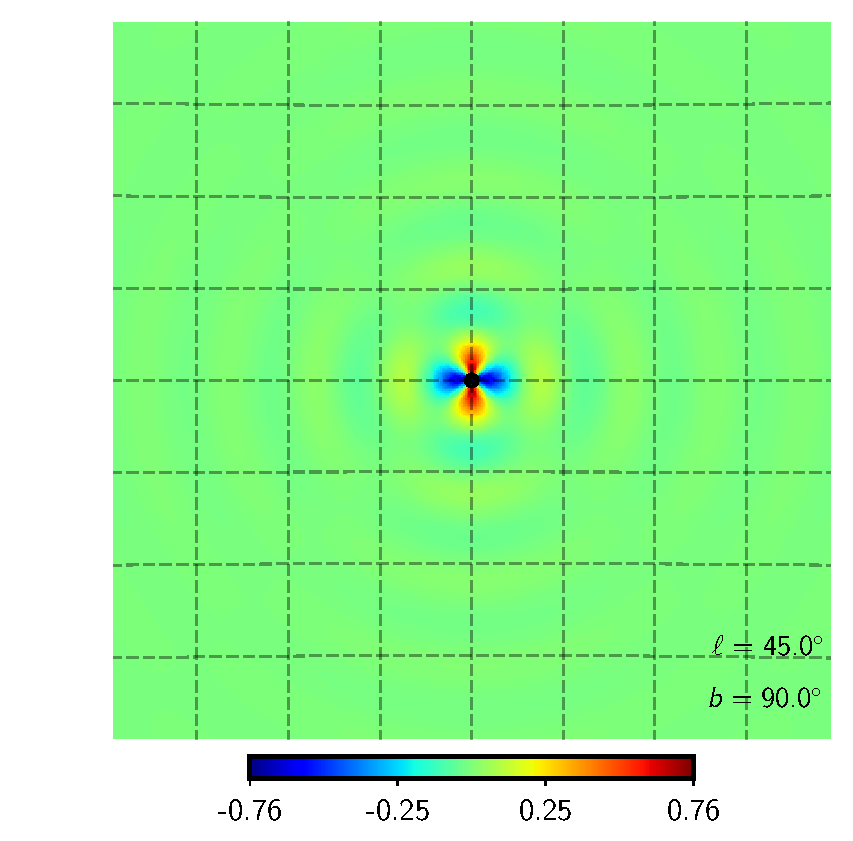
\includegraphics[width=0.16\columnwidth]{kernel/I_ker_r_lat90_lon45.pdf}}\hspace{-2mm}
\subfigure{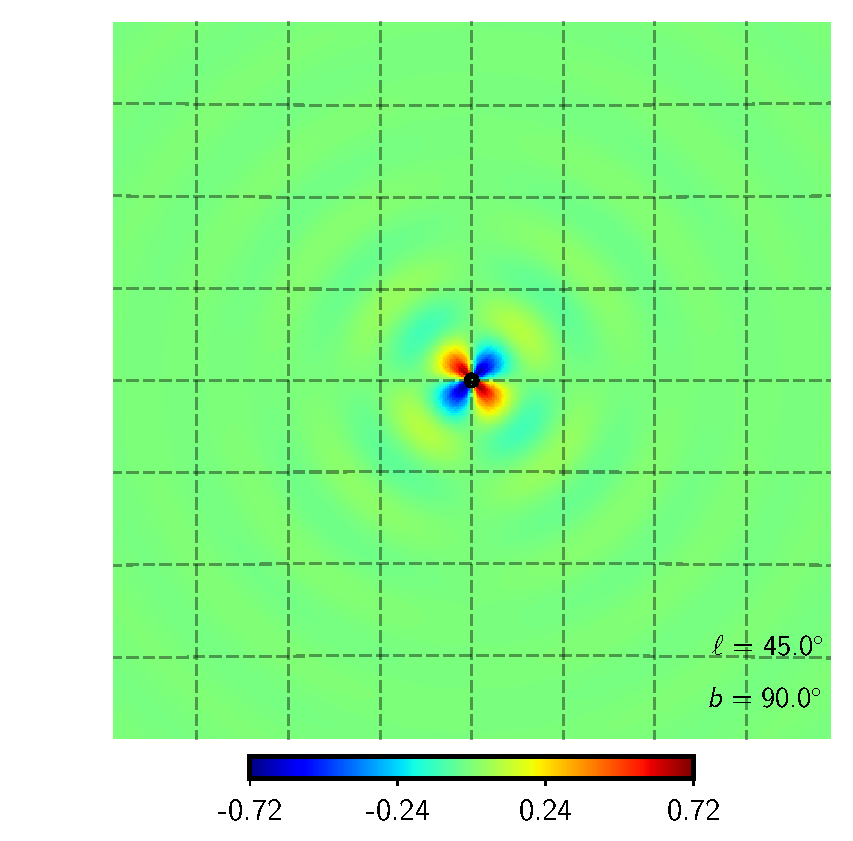
\includegraphics[width=0.16\columnwidth]{kernel/I_ker_i_lat90_lon45.pdf}}\\[-2ex]
\subfigure{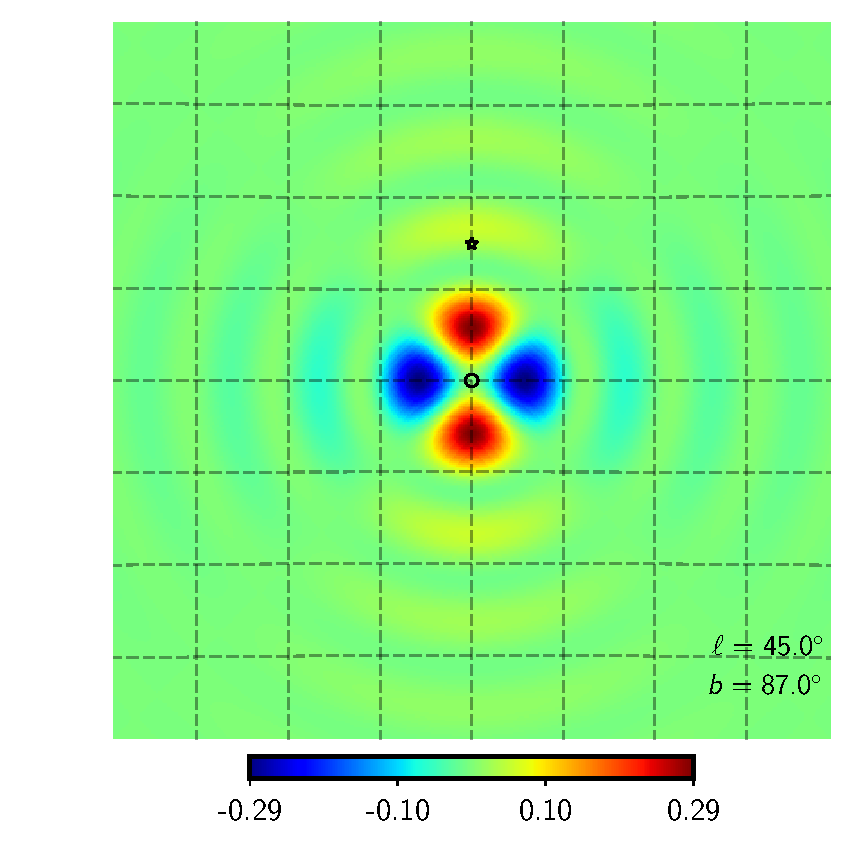
\includegraphics[width=0.16\columnwidth]{kernel/qu2eb_ker_r_lat87_lon45.pdf}}\hspace{-2mm}
\subfigure{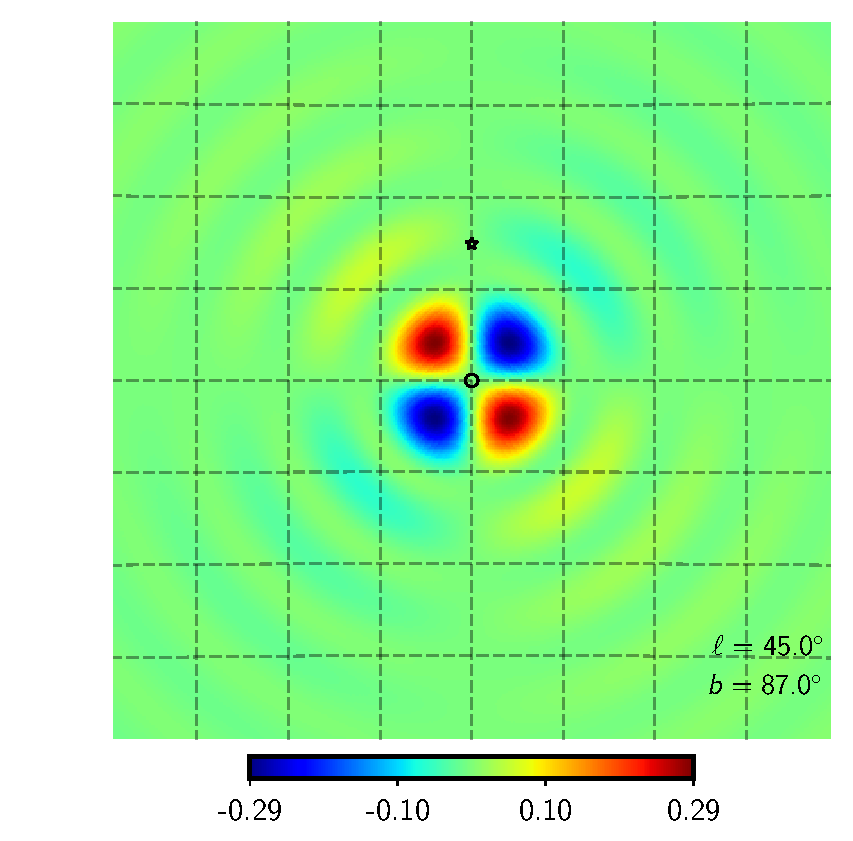
\includegraphics[width=0.16\columnwidth]{kernel/qu2eb_ker_i_lat87_lon45.pdf}}\hspace{-2mm}
\subfigure{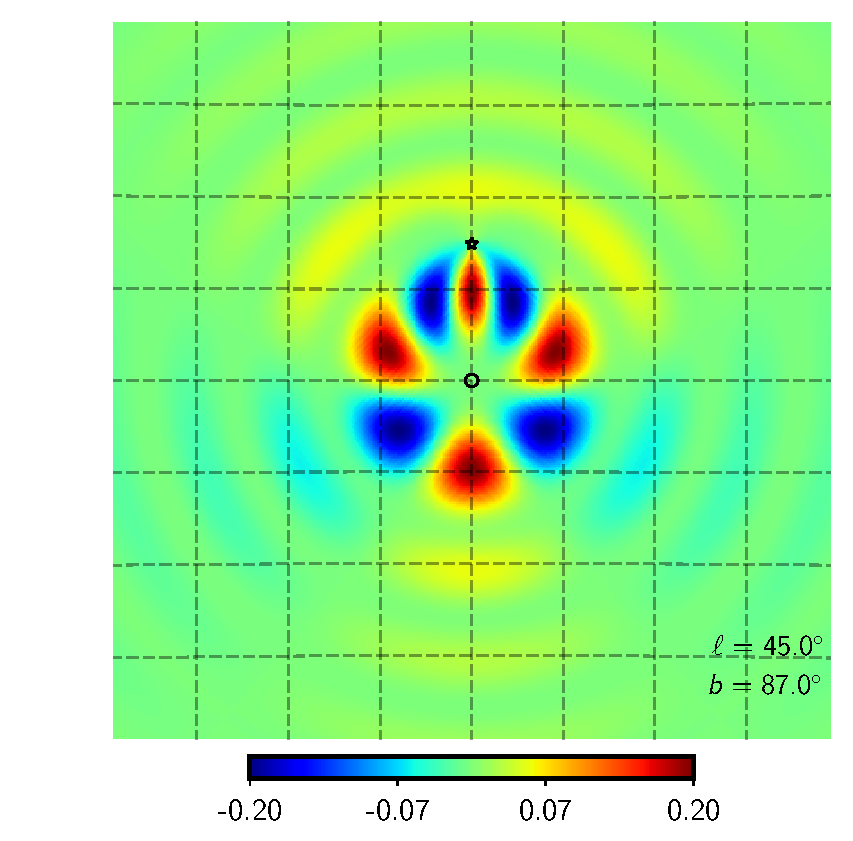
\includegraphics[width=0.16\columnwidth]{kernel/qu2ebqu_ker_r_lat87_lon45.pdf}}\hspace{-2mm}
\subfigure{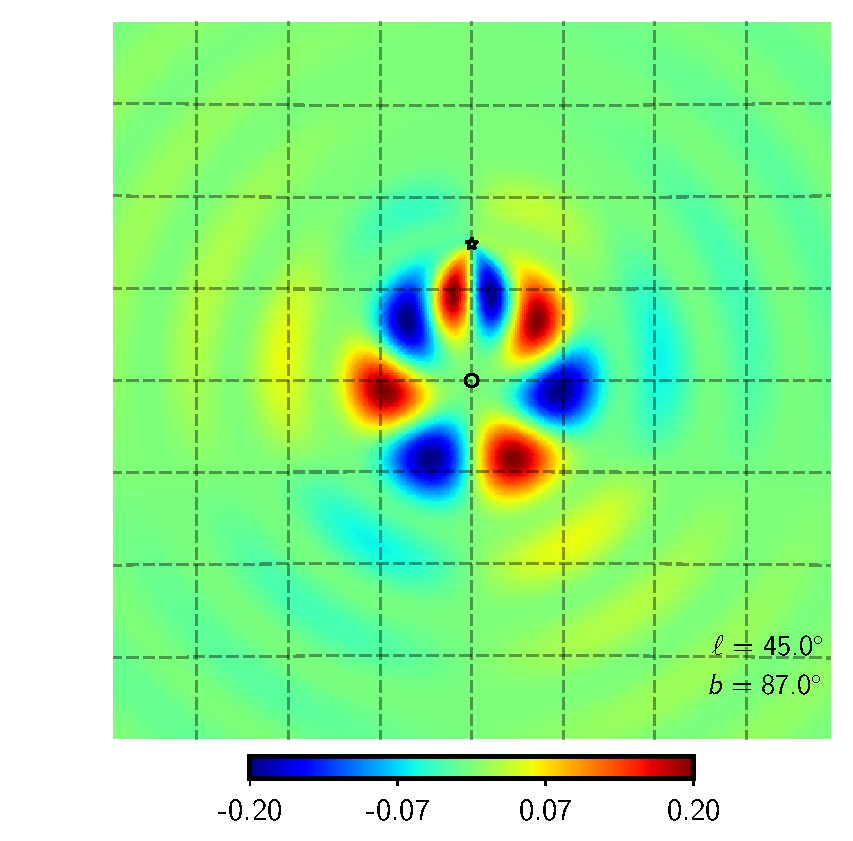
\includegraphics[width=0.16\columnwidth]{kernel/qu2ebqu_ker_i_lat87_lon45.pdf}}\hspace{-2mm}
\subfigure{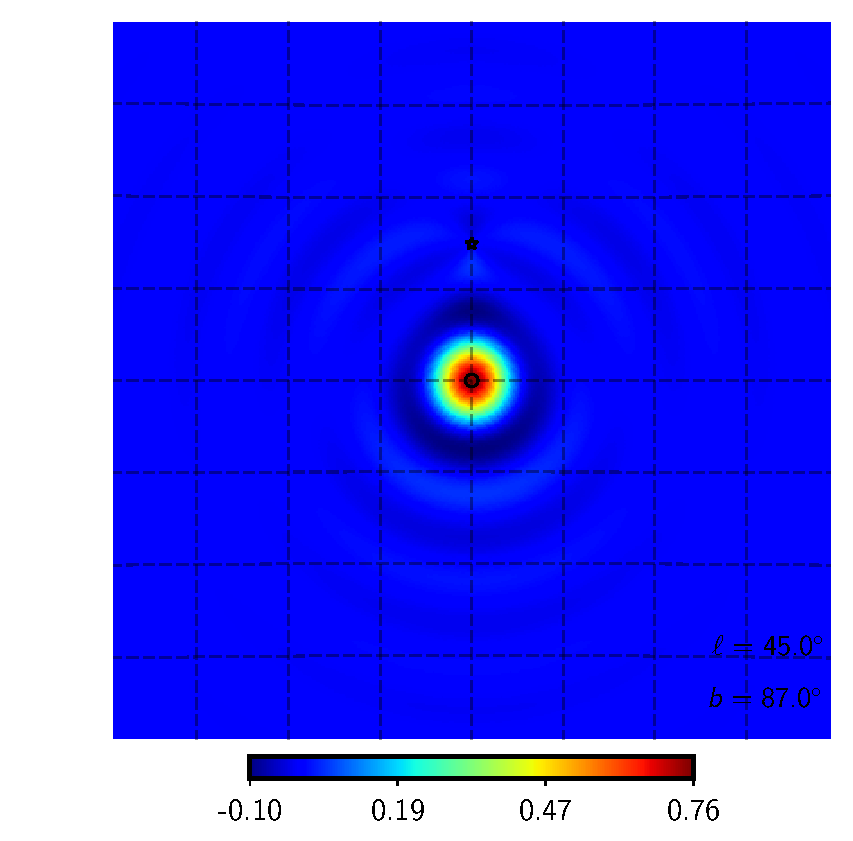
\includegraphics[width=0.16\columnwidth]{kernel/I_ker_r_lat87_lon45.pdf}}\hspace{-2mm}
\subfigure{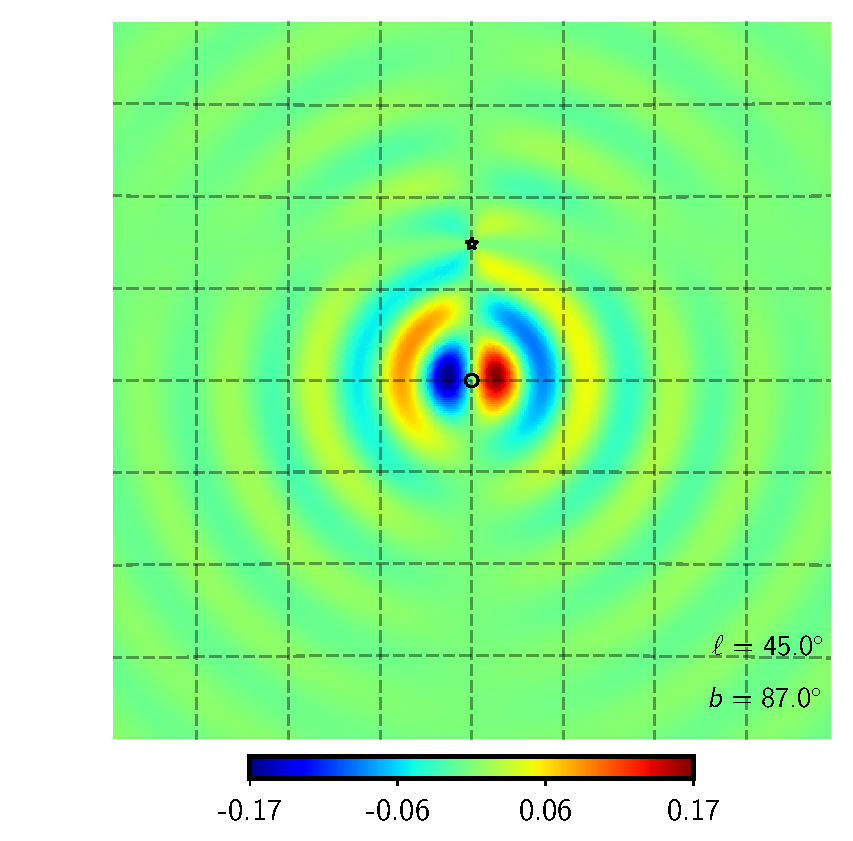
\includegraphics[width=0.16\columnwidth]{kernel/I_ker_i_lat87_lon45.pdf}}\\[-2ex]
\subfigure{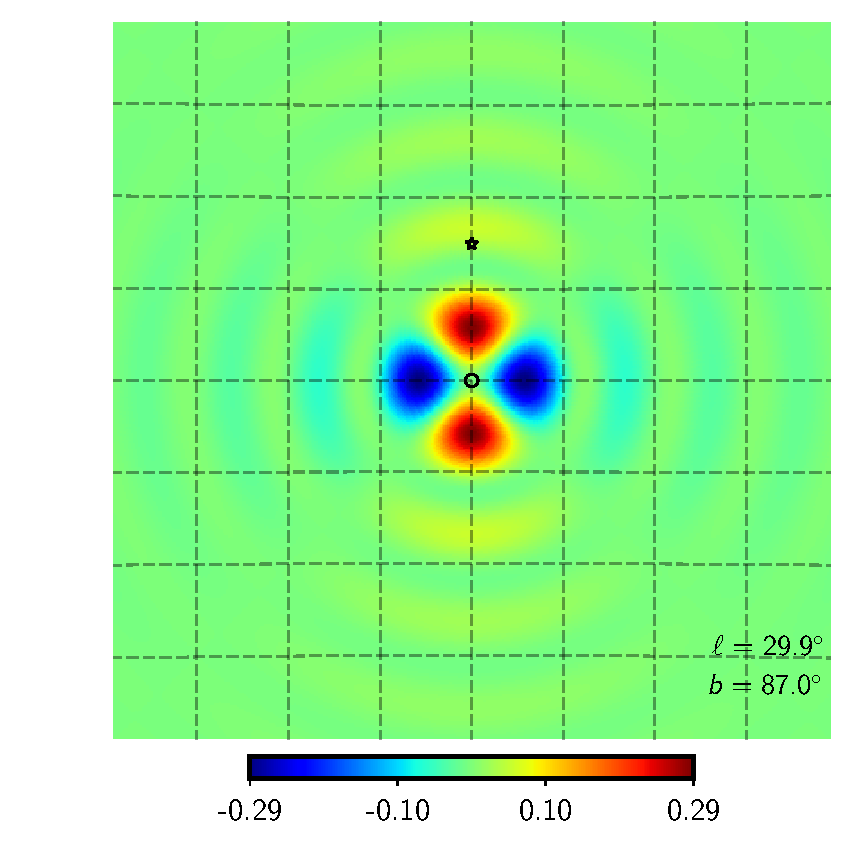
\includegraphics[width=0.16\columnwidth]{kernel/qu2eb_ker_r_lat87_lon30.pdf}}\hspace{-2mm}
\subfigure{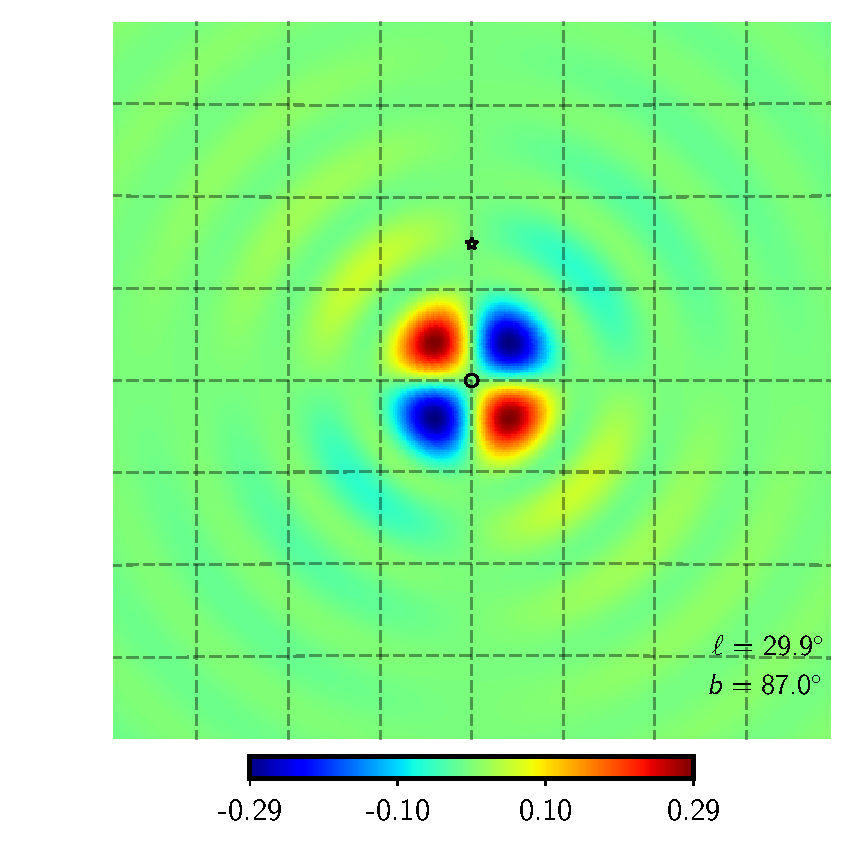
\includegraphics[width=0.16\columnwidth]{kernel/qu2eb_ker_i_lat87_lon30.pdf}}\hspace{-2mm}
\subfigure{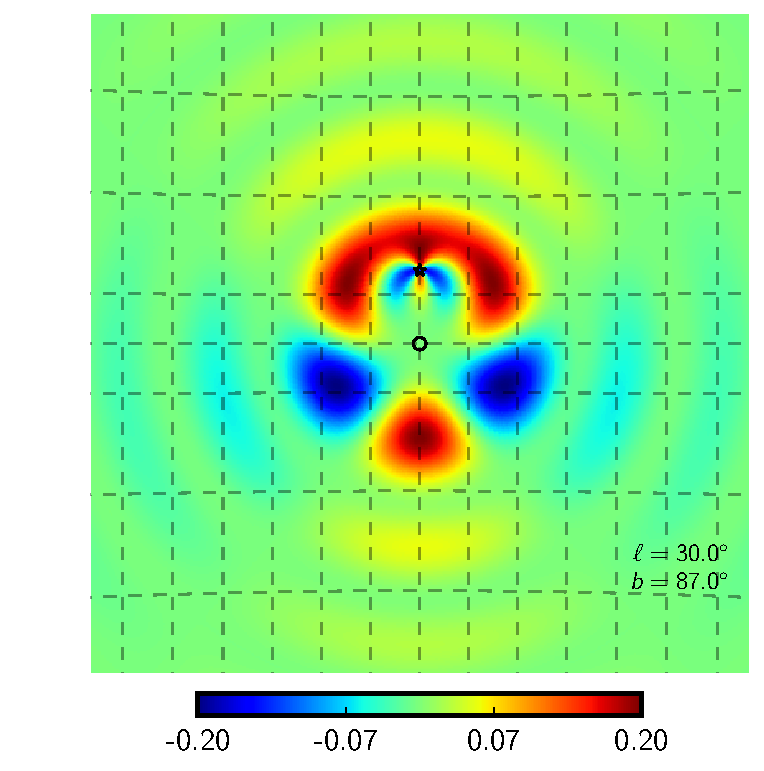
\includegraphics[width=0.16\columnwidth]{kernel/qu2ebqu_ker_r_lat87_lon30.pdf}}\hspace{-2mm}
\subfigure{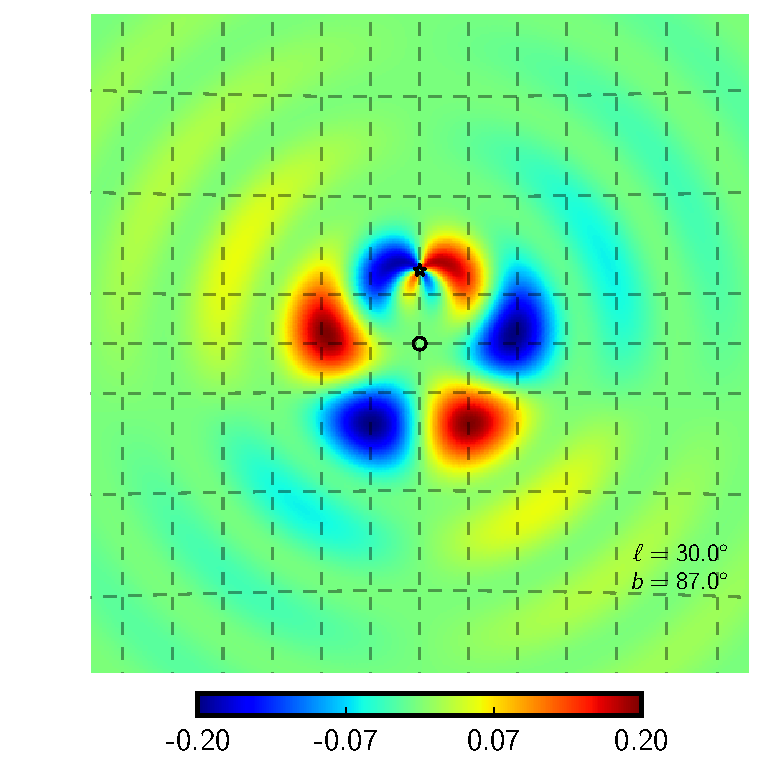
\includegraphics[width=0.16\columnwidth]{kernel/qu2ebqu_ker_i_lat87_lon30.pdf}}\hspace{-2mm}
\subfigure{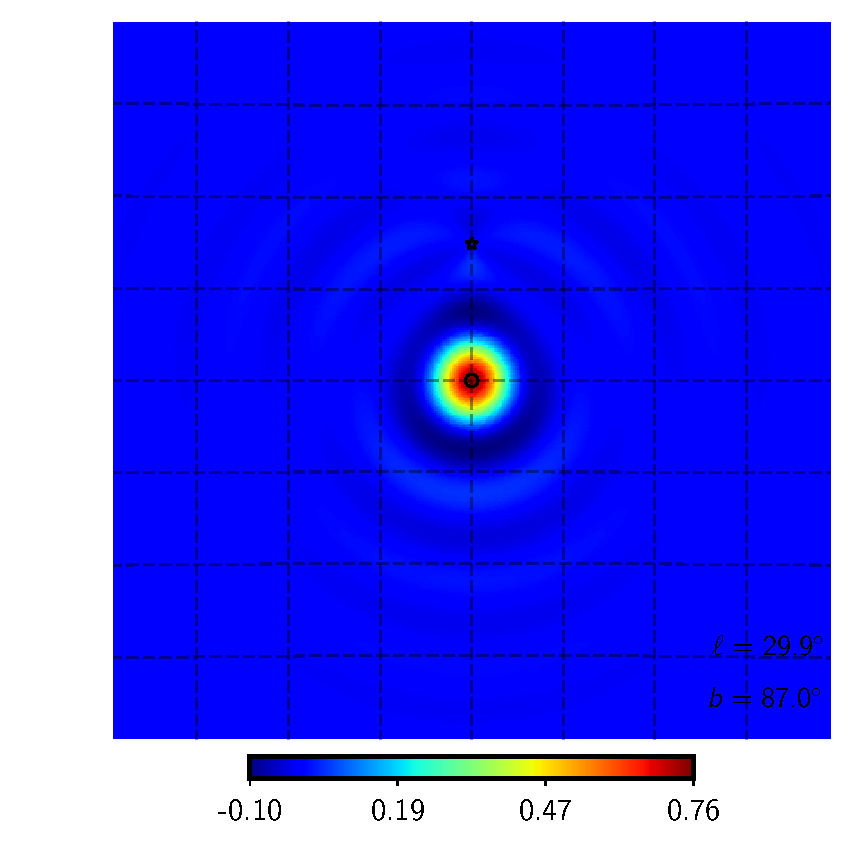
\includegraphics[width=0.16\columnwidth]{kernel/I_ker_r_lat87_lon30.pdf}}\hspace{-2mm}
\subfigure{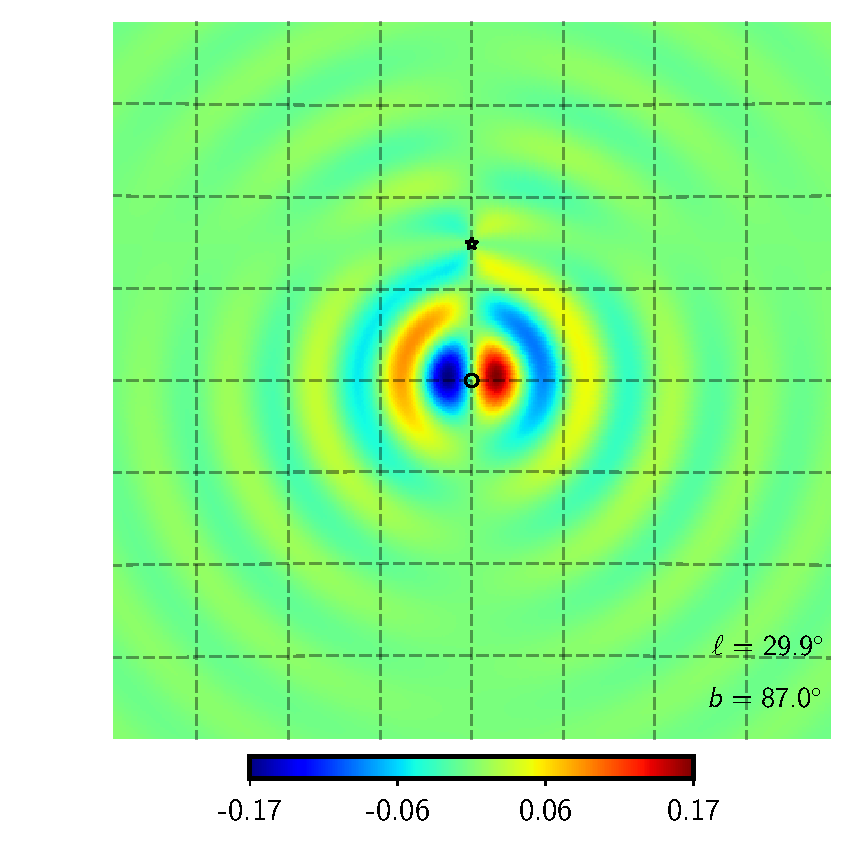
\includegraphics[width=0.16\columnwidth]{kernel/I_ker_i_lat87_lon30.pdf}}\\[-2ex]
\subfigure{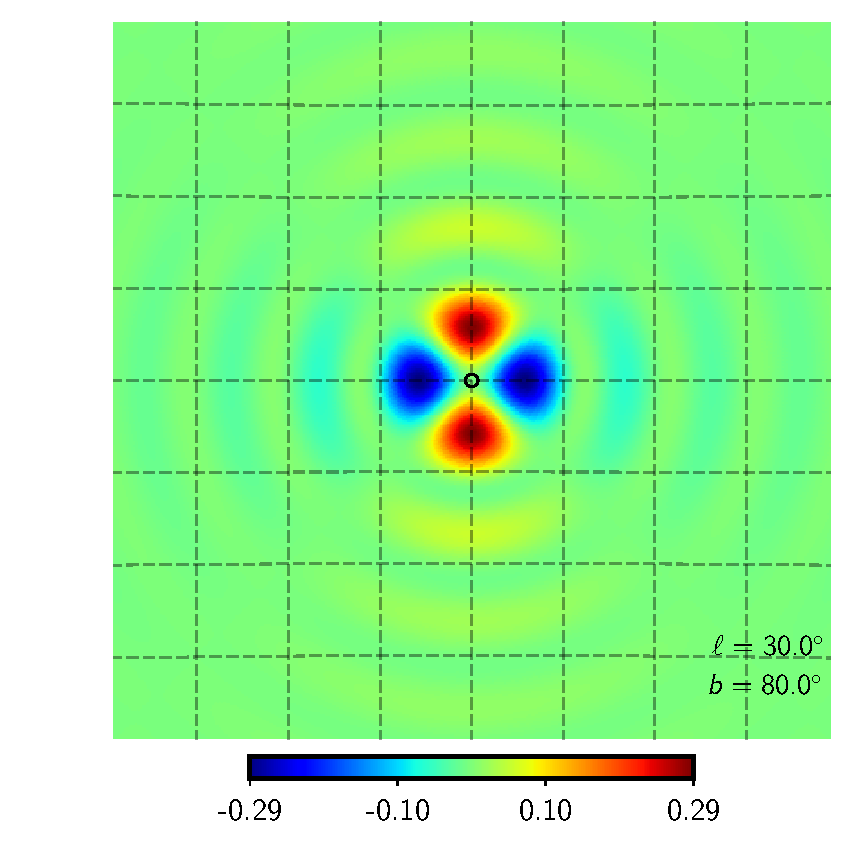
\includegraphics[width=0.16\columnwidth]{kernel/qu2eb_ker_r_lat80_lon30.pdf}}\hspace{-2mm}
\subfigure{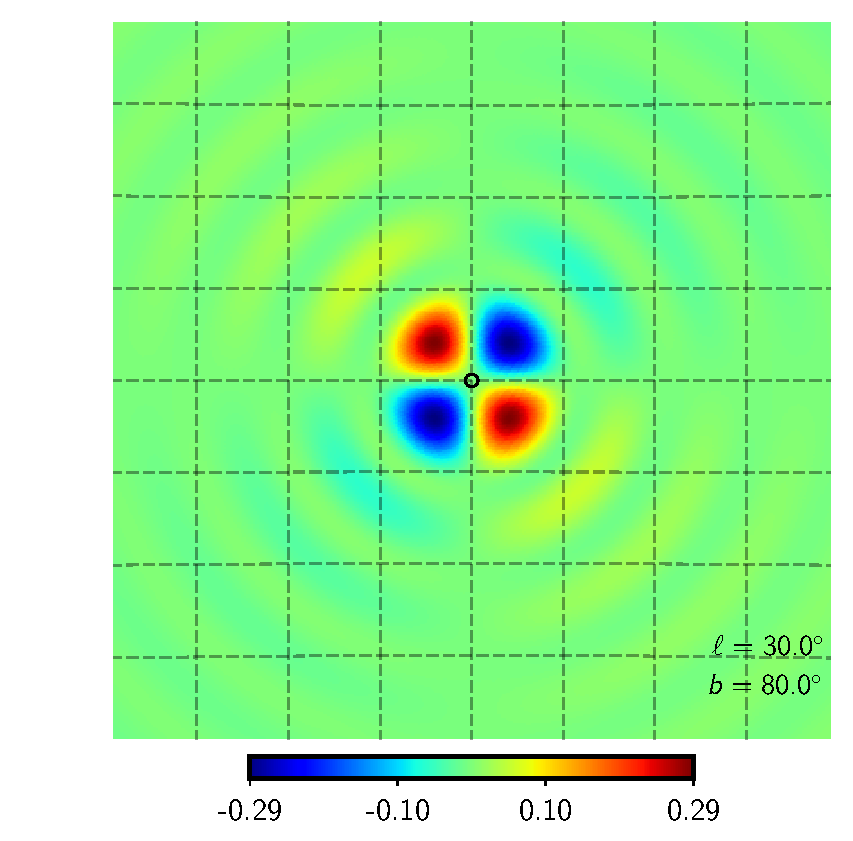
\includegraphics[width=0.16\columnwidth]{kernel/qu2eb_ker_i_lat80_lon30.pdf}}\hspace{-2mm}
\subfigure{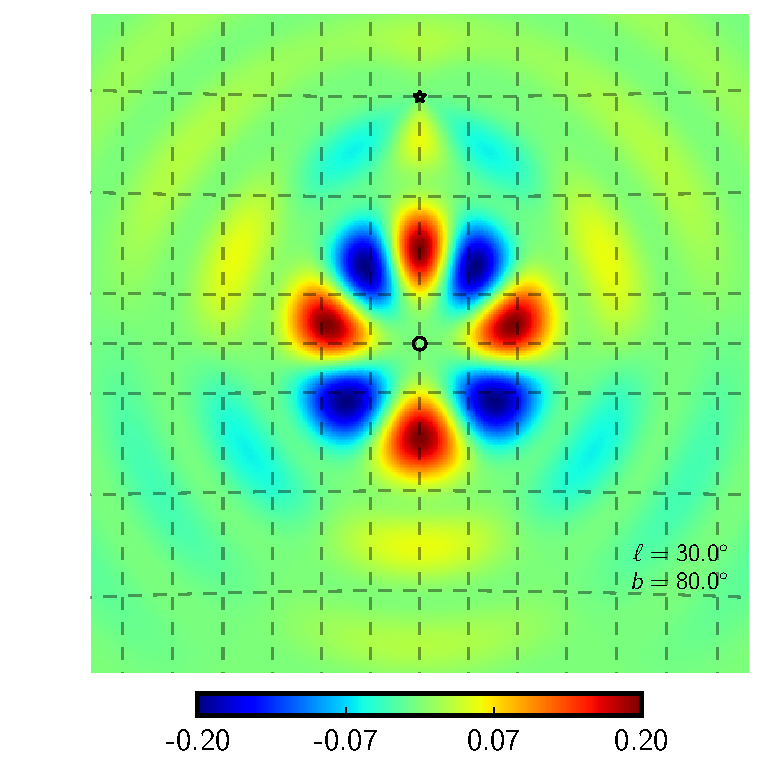
\includegraphics[width=0.16\columnwidth]{kernel/qu2ebqu_ker_r_lat80_lon30.pdf}}\hspace{-2mm}
\subfigure{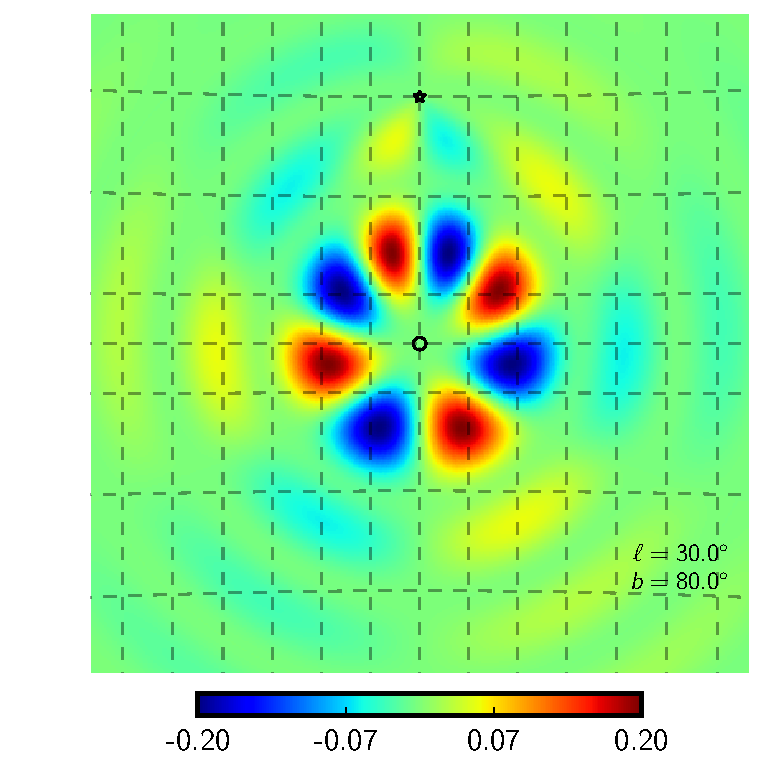
\includegraphics[width=0.16\columnwidth]{kernel/qu2ebqu_ker_i_lat80_lon30.pdf}}\hspace{-2mm}
\subfigure{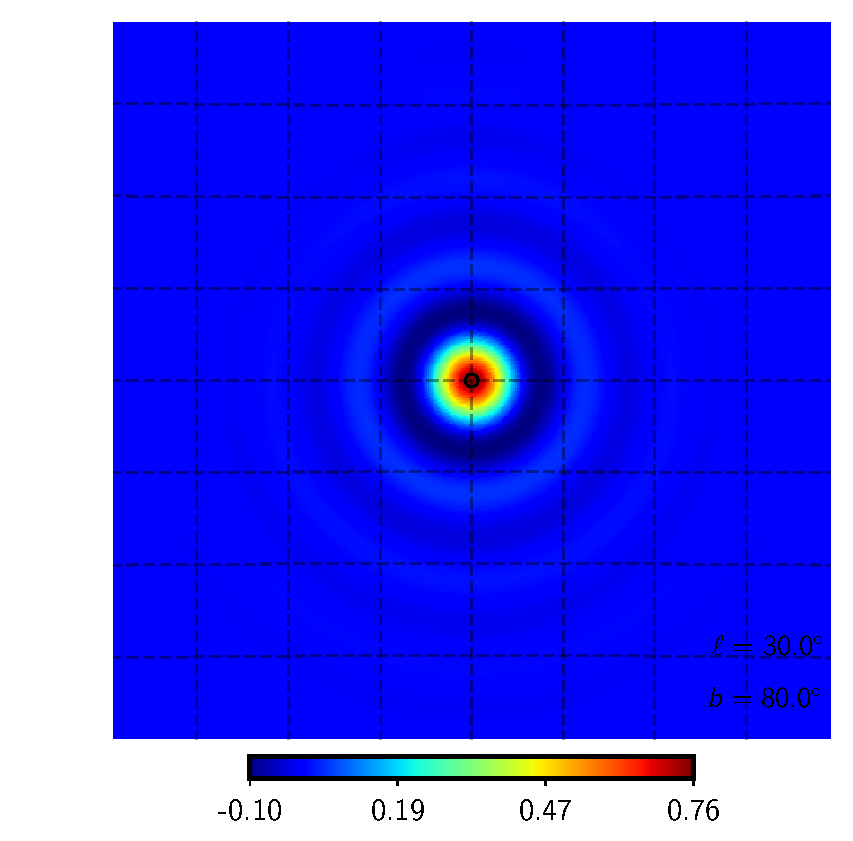
\includegraphics[width=0.16\columnwidth]{kernel/I_ker_r_lat80_lon30.pdf}}\hspace{-2mm}
\subfigure{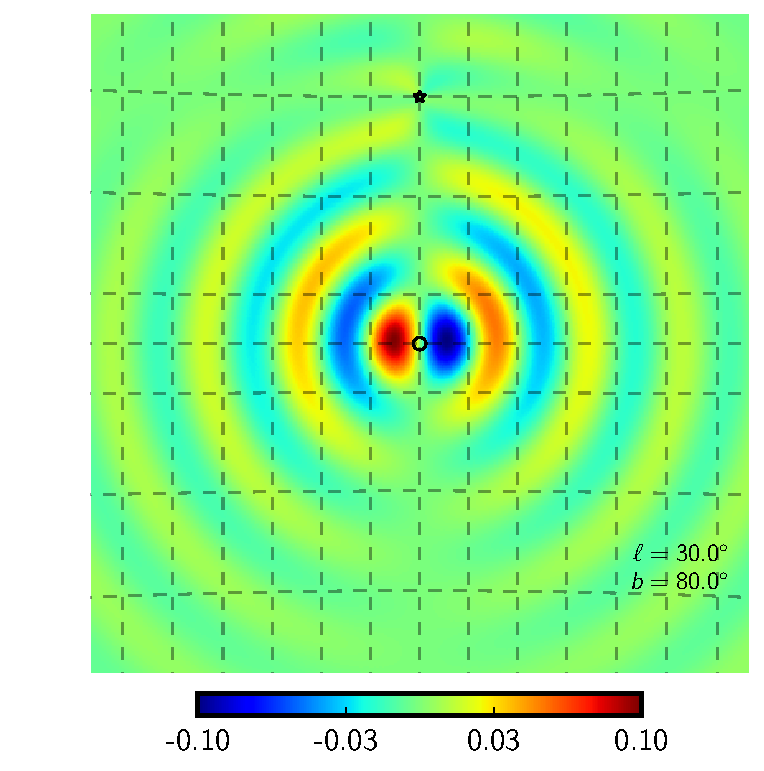
\includegraphics[width=0.16\columnwidth]{kernel/I_ker_i_lat80_lon30.pdf}}\\[-2ex]
\subfigure[$\mathcal{M}_r$]{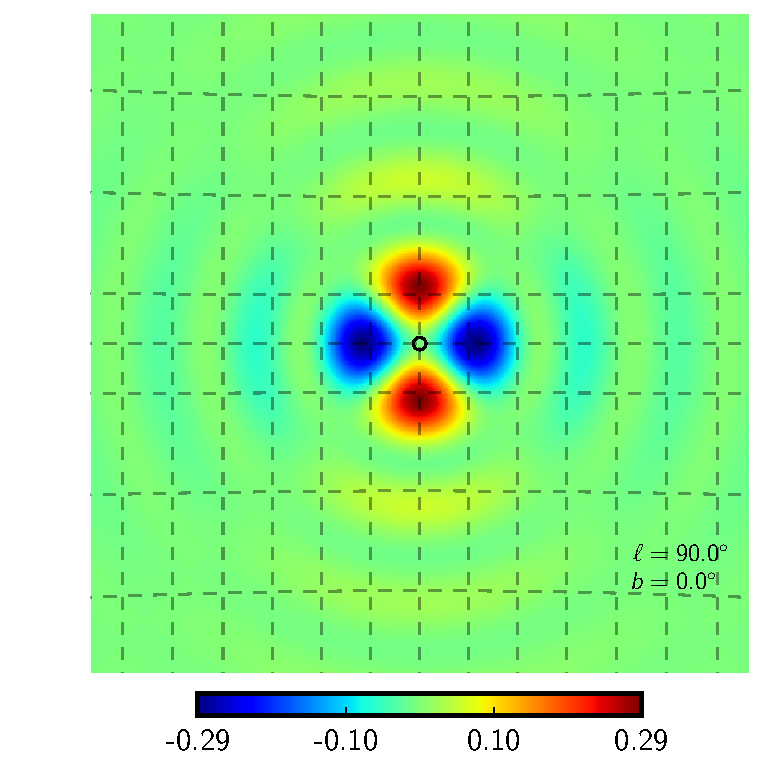
\includegraphics[width=0.16\columnwidth]{kernel/qu2eb_ker_r_lat0_lon90.pdf}}\hspace{-2mm}
\subfigure[$\mathcal{M}_i$]{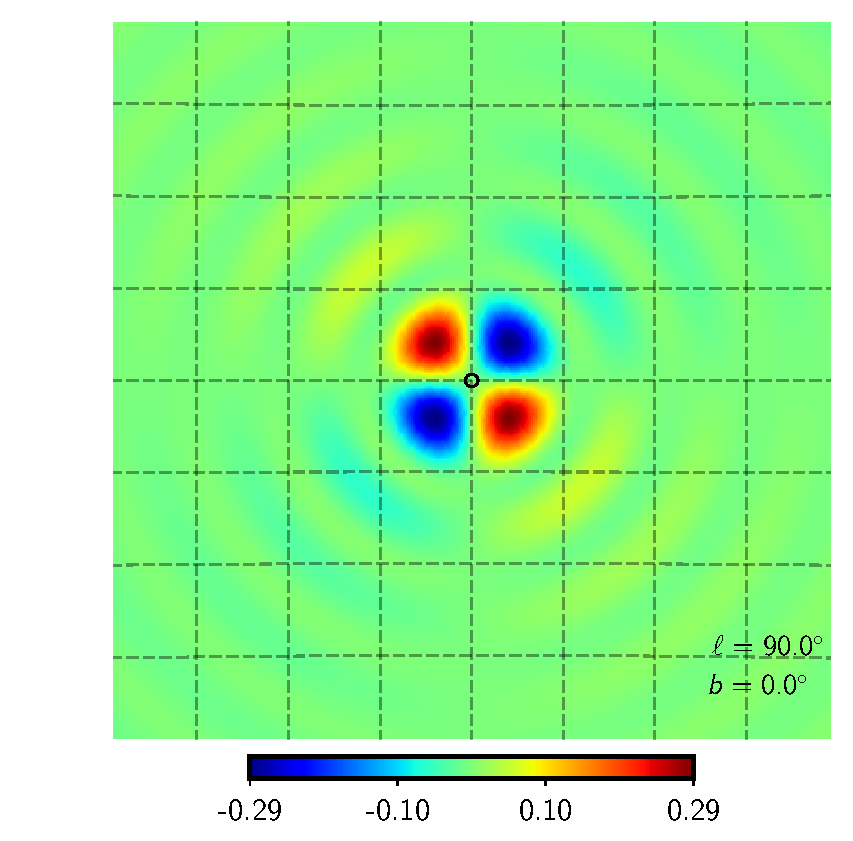
\includegraphics[width=0.16\columnwidth]{kernel/qu2eb_ker_i_lat0_lon90.pdf}}\hspace{-2mm}
\subfigure[$\mathcal{D}_r$]{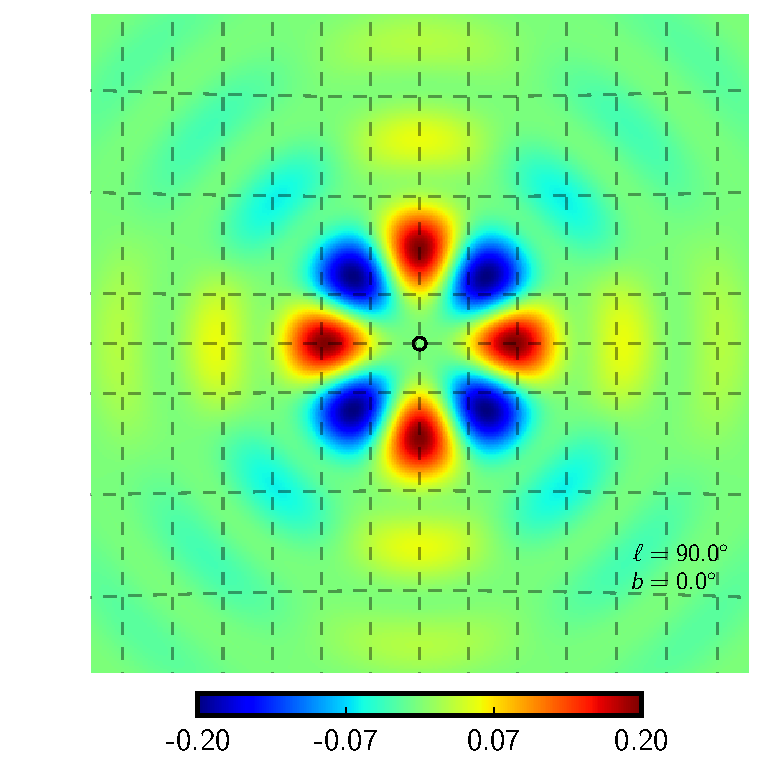
\includegraphics[width=0.16\columnwidth]{kernel/qu2ebqu_ker_r_lat0_lon90.pdf}}\hspace{-2mm}
\subfigure[$\mathcal{D}_i$]{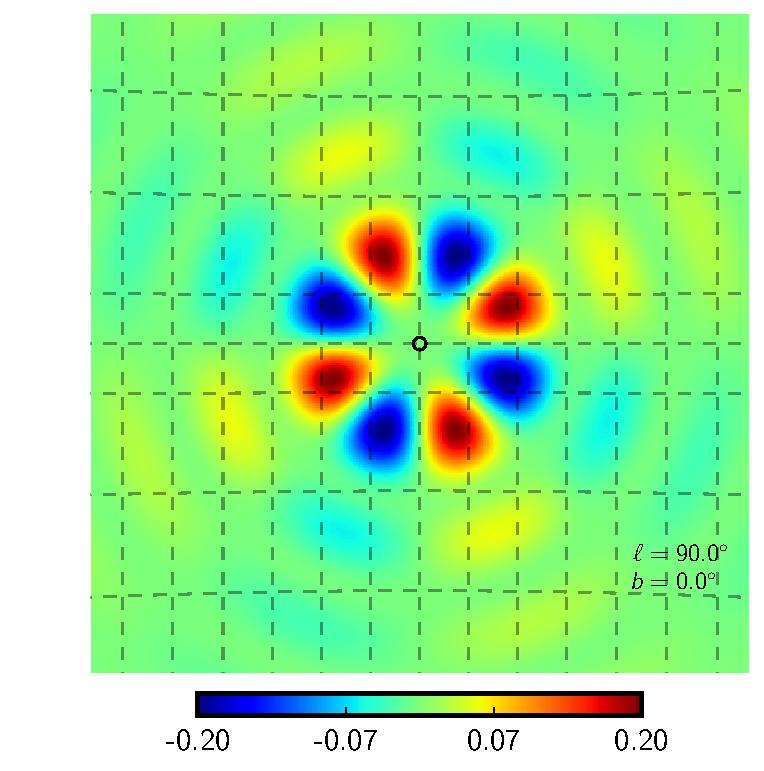
\includegraphics[width=0.16\columnwidth]{kernel/qu2ebqu_ker_i_lat0_lon90.pdf}}\hspace{-2mm}
\subfigure[$\mathcal{I}_r$]{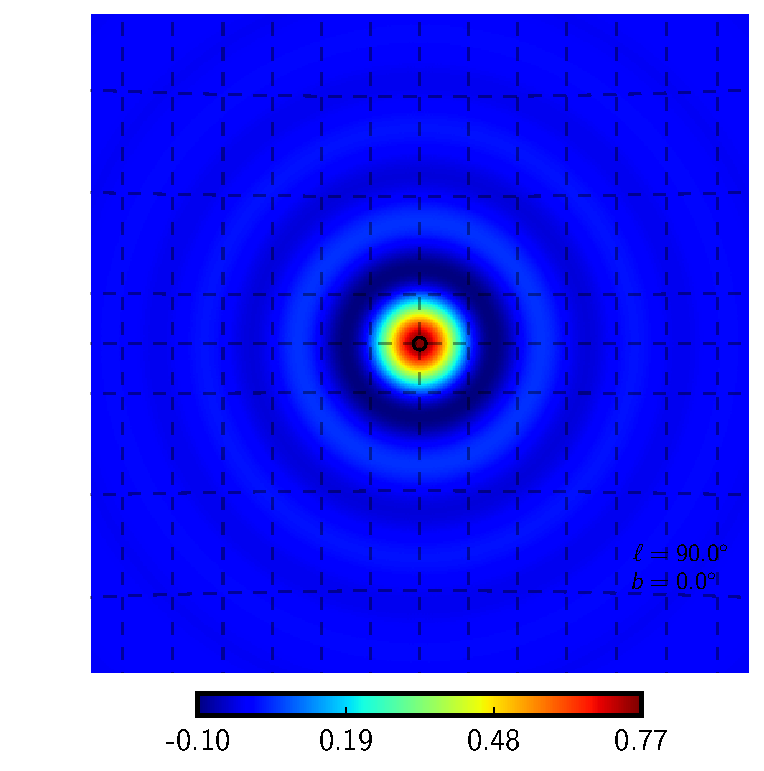
\includegraphics[width=0.16\columnwidth]{kernel/I_ker_r_lat0_lon90.pdf}}\hspace{-2mm}
\subfigure[$\mathcal{I}_i$]{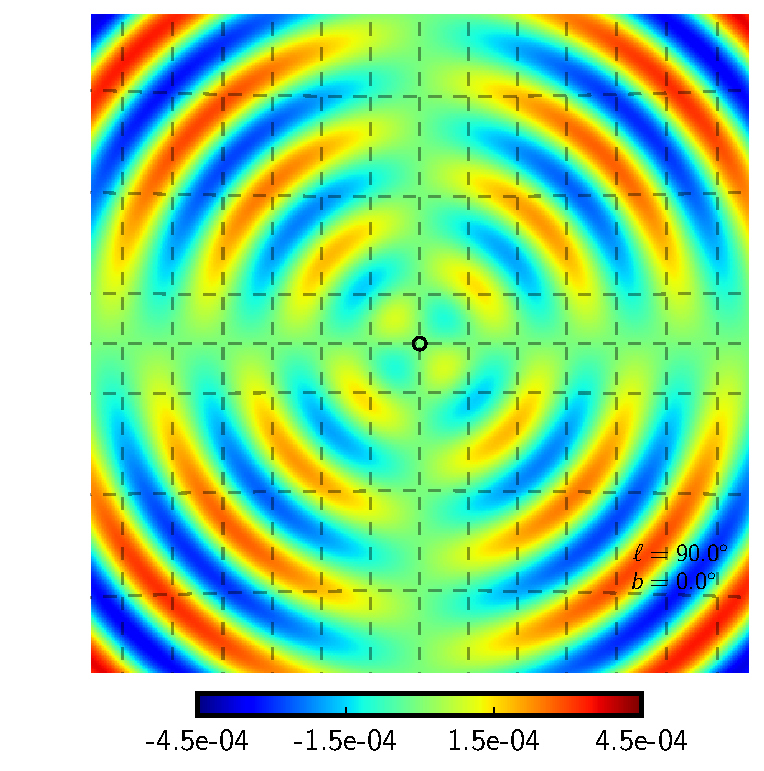
\includegraphics[width=0.16\columnwidth]{kernel/I_ker_i_lat0_lon90.pdf}}
\caption{This panel of figure depicts the various parts of the convolution kernel, discussed in \sec{sec:real_space_operators}. These kernels have been evaluated with the band limit: $\ell \in [2,192]$. The functions have been sampled at an NSIDE=2048 resolution for visual appeal. The size of each panel is approximately $16^{\circ} \times 16^{\circ}$ and the grid lines are marked at 2 degree separations. The black circles denotes the position of the central pixel around which the convolution kernels have been evaluated. The black star marks the location of the north galactic pole. The five rows depict the kernels at different location on the sphere and the galactic coordinates of the central pixel are specified in each panel. }
%from top to bottom rows are as follows $[b,\ell] = [0^{\circ},0^{\circ}], [87^{\circ},0^{\circ}], [87^{\circ},30^{\circ}], [80^{\circ},30^{\circ}], [0^{\circ},90^{\circ}]$.}
\label{fig:vis_kernel}
 \end{figure}
%
\revisit{Since its not easy to imagine how the Euler angles vary as a function of position of the central pixel, we evaluate and depict the kernels at different locations, to give a sense of how these kernels vary across the sphere.} For illustration these functions are sampled at a very high Healpix resolution parameter of NSIDE=2048. All the plots have been rotated such that the pixel around which the kernels are evaluated lies in the centre marked by the back circle. The results are depicted in \fig{fig:vis_kernel}. 

The function $\mathcal{M}$ is identical irrespective of changes in the galactic latitude and longitude of the central pixel. \st{The only contrasting locations are the poles (i.e. $|b|=90^{\circ}$), where the functions $\mathcal{M}_r$ \& $\mathcal{M}_i$ are rotated by $45^{\circ}$  as compared to the respective functions evaluated at locations where $|b|\neq 90^{\circ}$.} Also note that these functions are not distorted when a part of the domain overlaps with the poles, as can be seen in the first three rows of \fig{fig:vis_kernel}. Both these facts can be associated with the fact that this function does not depend on the Euler angle $\gamma$. \revisit{Recall that the angle $\gamma$ defines the rotation about the final z-axis which co-alligns the planar axes. Since the function $\mathcal{M}$ does not depend of this final orientation, it implies a rotational invariance of the fields constructed by convolving with this kernel.}

The function $\mathcal{D}$ varies significantly as a function of galactic latitude of the central pixel. It varies from having a two fold symmetry at the poles to having a four fold symmetry at the equator as seen in the middle two columns of \fig{fig:vis_kernel}. This change in behavior is primarily due to the  dependence on the Euler angle $\gamma$. When the central pixel is nearly at the pole, $\gamma$ vanishes, and the azimuthal part of the function $D$ is identical to that of $\mathcal{M}$ and hence the two function look very similar as seen in the first row of \fig{fig:vis_kernel}. Also note that this function is distorted as parts of its domain pass the galactic poles.  

The function $\mathcal{I}$ shows similar behavior, varying with latitude, having an identical azimuthal behavior near the poles and being distorted in parts that overlap with the galactic poles. \revisit{This function, in the case of an infinite band limit reduces to a delta function at the position of the central pixel ($\lim_{\ell_{\rm max} \to \infty}: \mathcal{I}_r \rightarrow \delta(\hat{n}_0 - \hat{n}'),~ \mathcal{I}_i \rightarrow 0$), as discussed previously.  Hints of this behavior can be seen by comparing the amplitudes of the real and imaginary parts of this function near the equator, depicted in the fifth row of the last two columns of \fig{fig:vis_kernel}. However note that this function significantly deviates from this behavior at higher galactic latitudes. The real and imaginary parts of this function contribute nearly equally near the vicinity of the poles.}  We invariably work with a specific band limit, hence both the real and imaginary parts of this functions make important non-zero contributions. 

We reiterate that all the function are invariant under changes in longitude of the central pixel, the latitude being held fixed as can be seen by comparing the figures in the second row (evaluated at $[b,\ell]=[87^{\circ},45^{\circ}]$) and third row (evaluated at $[b,\ell]=[87^{\circ},30^{\circ}]$) of \fig{fig:vis_kernel}, as one may have expected.

\subsection{Quantifying the non-locality of E \& B modes} \label{sec:radial_locality}
It is clear from previous discussions that that the non-locality of the E and B modes is determined by the radial part of the convolution kernels. To quantify this non-locality as a function of the maximum multipole accessible for analysis, we evaluate the radial part of the convolution kernel for different values of $\ell_{\rm max}$, while keeping the lowest multipole fixed at $\ell_{\rm min}=2$. 
%
\begin{figure}[t]
\centering
\subfigure{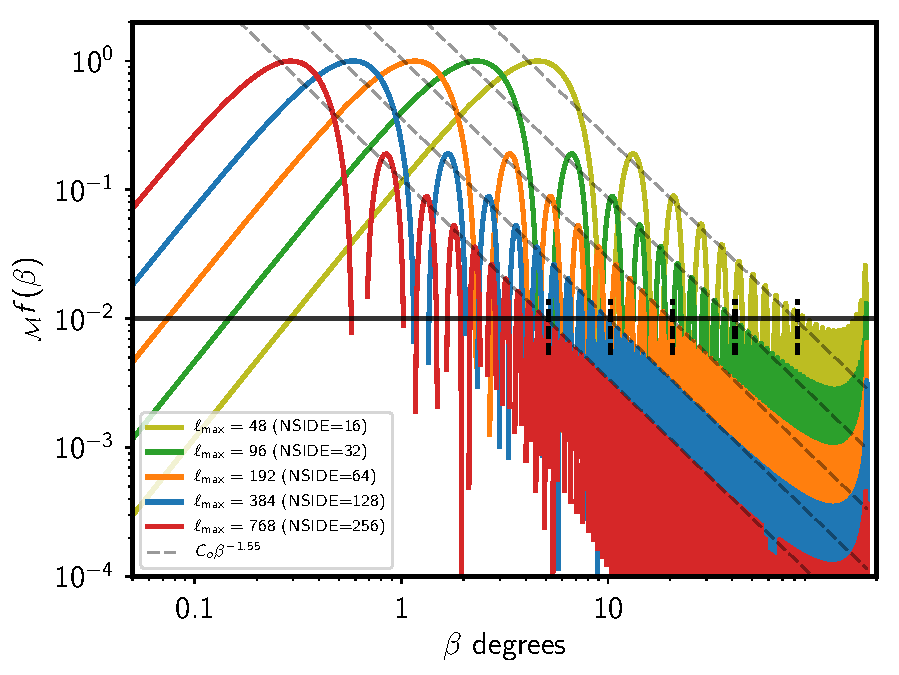
\includegraphics[width=0.96\columnwidth]{kernel/f_rad_ker_fn_of_ellmax.pdf}}
\subfigure{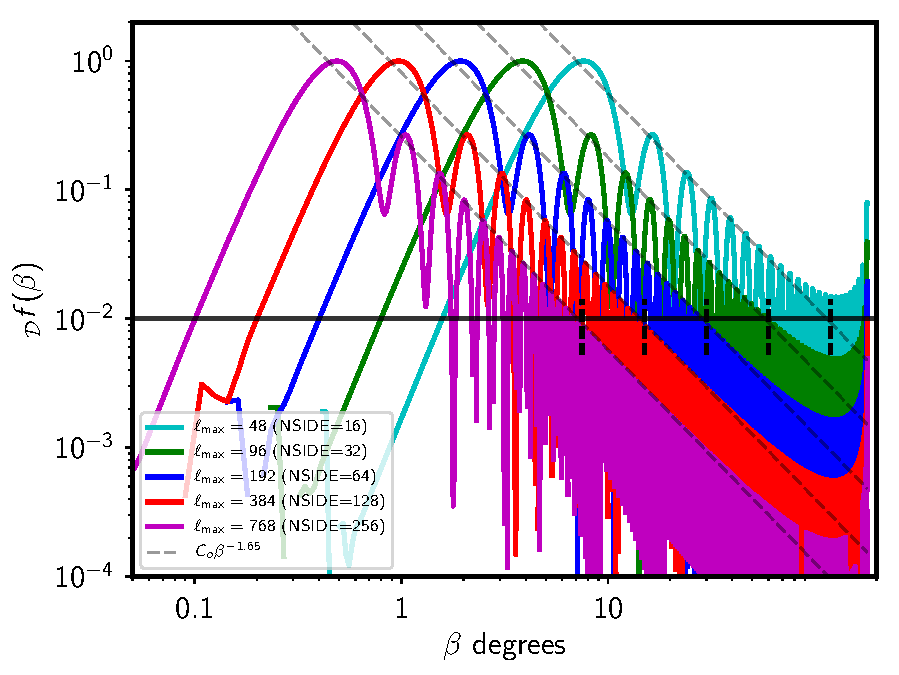
\includegraphics[width=0.48\columnwidth]{kernel/fp2_rad_ker_fn_of_ellmax.pdf}}
\subfigure{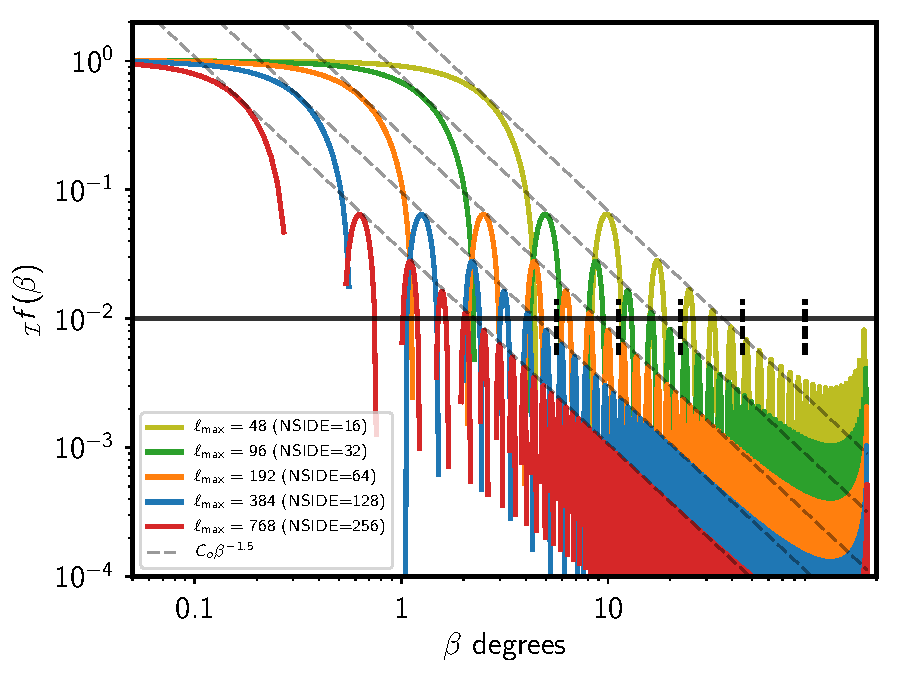
\includegraphics[width=0.48\columnwidth]{kernel/fm2_rad_ker_fn_of_ellmax.pdf}}
\caption{The top panel shows a plot of the radial kernels $f(\beta,\ell_{\rm min},\ell_{\rm max})$ while the bottom left and right panels show the radial functions ${}_{+2}f(\beta,\ell_{\rm min},\ell_{\rm max}) ~\&~ {}_{-2}f(\beta,\ell_{\rm min},\ell_{\rm max})$ respectively, for different $\ell_{\rm max}$ as indicated by the legends and fixed $\ell_{\rm min}=2$. The curves for each of these functions have been normalized such that the maximum of the curve is set to unity. The horizontal solid black line marks the location where the amplitude of the kernel falls below 1\% of its maximum. The slanted dashed black lines indicate a power law fit (by eye) to the envelope of the radial functions. While the envelopes for function $f(\beta)~\&~ {}_{-2}f(\beta)$ are fit well by the power law $\propto \beta^{-1.5}$, the envelope for the function ${}_{-2}f(\beta)$ is seen to have a slightly steeper fall off $\propto \beta^{-1.65}$.}
\label{fig:rad_ker_decay}
\end{figure}
%
The set of radial kernels so derived are plotted in \fig{fig:rad_ker_decay}. All the function have been normalized such that their global maxima is set to unity. Note that on increasing $\ell_{\rm max}$ the radial kernels shift to the left, attaining fractions of  their global maxima at progressively small angular distances $\beta$ from the central pixel.  

We have observed that the radial functions derived by evaluating the multipole sums to different maximum multipoles are self similar. Specifically these functions follow an interesting telescoping and scaling property: $${}_rf(\beta,2,\ell_{\rm max}) \approx \Big[\frac{\ell_{\rm max}}{\ell'_{\rm max}}\Big]^2{}_rf(\beta'=\frac{\ell_{\rm max}}{\ell'_{\rm max}} \beta ,2,\ell'_{\rm max}) \,,$$ where ${}_rf$ denotes all the different radial functions. We can understand the shifting left of the radial kernels on increasing the maximum multipole using this property. Lets say the function ${}_rf(\beta, \ell'_{\rm max})$ transition to being monotonously below some fraction of the global maxima at an angular distance of $\beta_0$.  The function ${}_rf(\beta', \ell_{\rm max})$, given $\ell_{\rm max} > \ell'_{\rm max}$, reaches the same transition point $\beta'=\beta_0$ at a smaller value of $\beta$ owing to the fact that $\ell_{\rm max}/\ell'_{\rm max}$ is greater than unity. The amplitude scaling of the functions is irrelevant since the transition point is always described in terms of the fraction of the global maxima of the function.

We are primarily interested in the non-local dependence of the scalar modes E \& B on the Stokes parameters Q \& U. We define the value of the abscissa at which the function $f(\beta,\ell_{\rm min},\ell_{\rm max})$ transits to being monotonously below 1\% of the maxima of the function as the non-locality parameter: $\beta_{o}$.  For a $\ell_{\rm max}=24$, the maximum multipole accessible on a Nside=8 Healpix map, the non-locality parameter $\beta_0=180^{\circ}$, since the radial function never falls monotonously below 1\% of the global maxima of the function. Using the self similar  property of the radial function discussed above, we define the following: $\beta_o= {\rm min}(180,180 \frac{24}{\ell_{\rm max}})$ as the non-locality parameter, given the maximum multipole $\ell_{\rm max}$. \revisit{$\beta_0$ is not very sensitive to $\ell_{\rm min}$, though it can be important on making drastic changes to $\ell_{\rm min}$. } \comment{Quantify how changing $\ell_{\rm min}$ changes $\beta_0$}

The envelope of the radial kernel $f(\beta,\ell_{\rm min},\ell_{\rm max})$ is observed to have a power law relation to the angular distance $\beta$ as seen in \fig{fig:rad_ker_decay}. At small values of $\beta$, which corresponds to the flat sky limit,  the radial function is proportional to $\beta^2$. In the intermediate range,  a fit by eye indicates that the envelope of the function is well represented by the power law $\beta^{-1.5}$.
\comment{There isn't too much of a discussion surrounding the function ${}_{\pm}f(\beta)$.}